% gCOVguide.tex
% v4.0 released February 2015

\documentclass{gCOV2e}

\usepackage{epstopdf}% To incorporate .eps illustrations using PDFLaTeX, etc.
\usepackage{subfigure}% Support for small, `sub' figures and tables

\theoremstyle{plain}% Theorem-like structures
\newtheorem{theorem}{Theorem}[section]
\newtheorem{corollary}[theorem]{Corollary}
\newtheorem{lemma}[theorem]{Lemma}
\newtheorem{proposition}[theorem]{Proposition}

\theoremstyle{definition}
\newtheorem{definition}[theorem]{Definition}
\newtheorem{example}[theorem]{Example}

\theoremstyle{remark}
\newtheorem{remark}[theorem]{Remark}

\begin{document}

%\jvol{00} \jnum{00} \jyear{2015} \jmonth{February}

\articletype{GUIDE}

\title{\textit{Complex Variables and Elliptic Equations} \LaTeX\ guide for authors (Style 2 + NLM reference style)}

\author{
\name{D.A. Gerasimov\textsuperscript{a}$^{\ast}$\thanks{$^\ast$Corresponding author. Email: the.dmitrii.g@gmail.com}
and I.T. Consultant\textsuperscript{b}}
\affil{\textsuperscript{a}Taylor \& Francis, 4 Park Square, Milton Park, Abingdon, UK;
\textsuperscript{b}Institut f\"{u}r Informatik, Albert-Ludwigs-Universit\"{a}t, Freiburg, Germany}
\received{v4.0 released February 2015}
}

\maketitle

\begin{abstract}
This guide is for authors who are preparing papers for \textit{Complex Variables and Elliptic Equations} (\textit{gCOV})
using the \LaTeX\ document preparation system and the class file \texttt{gCOV2e.cls},
which is available via the journal's home page on the Taylor \& Francis website.
\end{abstract}

\begin{keywords}
submission instructions; source file coding; environments; references citation; fonts; numbering
\textbf{(Please provide three to six keywords taken from terms used in your manuscript)}
\end{keywords}

\begin{classcode}F1.1; F4.3 \textbf{(... for example; authors are encouraged to provide two to six 2010 Mathematics Subject Classification codes)}\end{classcode}


{\abstractfont\centerline{\bfseries Index to information contained in this guide}\vspace{12pt}
\hbox to \textwidth{\hsize\textwidth\vbox{\hsize17pc
\hspace*{-12pt} {1.}    Introduction\\
\hspace*{7pt} {1.1.}  The \textit{gCOV} document class\\
\hspace*{7pt} {1.2.}  Submission of \LaTeX\ articles\\
\hspace*{24pt}        to the journal\\
{2.}    Using the \textit{gCOV} class file\\
{3.}    Additional features\\
\hspace*{10pt}{3.1.}  Title, authors' names, abstract\\
\hspace*{24pt}        and keywords\\
\hspace*{10pt}{3.2.}  Additional footnotes to the\\
\hspace*{24pt}        title or authors' names\\
\hspace*{10pt}{3.3.}  Lists\\
{4.}    Some guidelines for using\\
\hspace*{6pt}        standard features\\
\hspace*{10pt}{4.1.}  Sections\\
\hspace*{10pt}{4.2.}  Illustrations (figures)\\
\hspace*{10pt}{4.3.}  Tables\\
\hspace*{10pt}{4.4.}  Landscape pages\\
\hspace*{10pt}{4.5.}   Theorem-like environments\\
\noindent \hspace*{7pt} {4.6.}   Typesetting mathematics\\
\hspace*{24pt} {4.6.1.}  Displayed mathematics\\
\hspace*{24pt} {4.6.2.}  Bold math italic symbols\\
\hspace*{24pt} {4.6.3.}  Bold Greek\\
\hspace*{24pt} {4.6.4.}  Upright Greek characters \\
\hspace*{47pt}            and the upright partial \\
\hspace*{47pt}            derivative sign }
\hspace{-24pt}\vbox{\noindent\hsize17pc
\hspace*{7pt} {4.7.}   Acknowledgements \\
\hspace*{7pt} {4.8.}   Disclosure \\
\hspace*{7pt} {4.9.}   Funding \\
\hspace*{7pt} {4.10.}   Notes \\
\hspace*{7pt} {4.11.}   Supplemental material \\
\hspace*{7pt} {4.12.}   References \\
\hspace*{24pt} {4.12.1.}  References cited in the \\
\hspace*{52pt}            text\\
\hspace*{24pt} {4.12.2.}  The list of references\\
\hspace*{7pt} {4.13.}   Appendices \\
{5.}    Example of a section heading \\*
\hspace*{6pt}   including {\fontencoding{T1}\scshape{small caps}}, \textit{italic}, \\
\hspace*{6pt}   and bold Greek such as ${\bm\kappa}$ \\
{6.}    \textit{gCOV} journal style \\
\hspace*{10pt}{6.1.}   Hyphens, en rules, em rules \\ \hspace*{27pt}and minus signs\\
\hspace*{10pt}{6.2.}   References \\
\hspace*{10pt}{6.3.}   Maths fonts\\
{7.}    Troubleshooting\\
{8.}    Fixes for coding problems\\
{9.}    Obtaining the \texttt{gCOV2e} class file\\
\hspace*{10pt}{9.1}  Via the Taylor \& Francis \\
\hspace*{24pt}       website\\
\hspace*{10pt}{9.2}  Via e-mail\\}}}


\section{Introduction}

????? 

\section{Definitions and notation}

\subsection{Notation}

\begin{itemize}
\item $\mathbb{C}$: complex plane, $\mathbb{C} = \{ x + \mathrm{i} y \mid x, y \in \mathbb{R} \}$ 
\item $\mathbb{H}$: upper complex half-plane, $\mathbb{H} = \{ x + \mathrm{i} y \mid y > 0, x, y \in \mathbb{R} \}$
\item $\mathbb{D}$: unit disk, $\mathbb{D} = \{ z \mid \left|z\right| < 1 \}$
\item $\mathbb{T}$: unit circle, $\mathbb{T} = \partial \mathbb{D} =  \{z \mid \left|z\right| = 1 \}$
\item $z$ denotes a complex argument on complex plane $\mathbb{C}$
\item $\zeta$ denotes a complex argument on unit disk $\mathbb{D}$
\end{itemize}

\subsection{Cayley transform}

Cayley transform maps $\mathbb{H}$ to $\mathbb{D}$:
\[
W(z) = \frac{z - \mathrm{i}}{z + \mathrm{i}}
\]
, whereas inverse Cayley transform maps $\mathbb{D}$ to $\mathbb{H}$:
\begin{equation}\label{eq:cayley_inverse}
w(\zeta) = \mathrm{i} \frac{1 + \zeta}{1 - \zeta}
\end{equation}

One notable property of the Cayley transform is that it injectively maps $\mathbb{R}$ into unit circle $\mathbb{T}$.

Another important property we are going to use is that Cayley transform preserves circles. In particular, a circle with radius $0 < r < 1$ centered in zero, under inverse Cayley transform maps into a circle with center $\mathrm{i} C(r)$ and radius $R(r)$, where:

\begin{equation}\label{eq:c_and_r}
\begin{aligned}
   C(r) &= \operatorname{Im} \frac{w(r) + w(-r)}{2} = \frac{1 + r^2}{1 - r^2}
\\ R(r) &= \operatorname{Im} \frac{w(r) - w(-r)}{2} = \frac{2 r}{1 - r^2}
\end{aligned}
\end{equation}

From these formulas it's easy to see that as $r$ approaches $1$, $R(r)$ goes to infinity and $C(r)$ converges to $R(r)$.

Also, we'll note two useful facts:
\begin{subequations}
\begin{equation}
C(r) - R(r) = \frac{(1 - r)^2}{1 - r^2} > 0
\label{eq:cr_positive}
\end{equation}
\begin{equation}
C(r) - R(r) = \frac{1 - r}{1 + r} < \frac{1}{R(r)} = \frac{1 - r^2}{2 r} \implies C - R \text{\ is\ } \mathcal{O}\left(\frac{1}{R}\right)
\label{eq:cr_small}
\end{equation}
\end{subequations}

\subsection{S-matrix}\label{sec:smatrix}
Consider a localized one dimensional potential barrier or resonator. We assume that the system evolves under the stationary Schrodinger's equation. Since we are only interested in the mathematical scattering problem and scattering state solutions, we set Plank's constant to $1$.

From the left and right we subject in to beams of quantum particles with the wavevector $k$, which will be a scalar in 1D case. Outside the potential barrier the particles behave as plane waves:

\begin{equation}\label{eq:wlwl}
\begin{aligned}
   \psi_L(x) &= A e^{\mathrm{i} k x} + B e^{-\mathrm{i} k x}
\\ \psi_R(x) &= C e^{\mathrm{i} k x} + D e^{-\mathrm{i} k x}
\end{aligned}
\end{equation}

S-matrix, or scattering matrix relates the final and initial states of the system:
\begin{equation}\label{eq:smatrix}
\begin{pmatrix} B \\ C \end{pmatrix} = S \begin{pmatrix} A \\ D \end{pmatrix}
\end{equation}
, and defines scattering properties of a potential barrier.

\section{Convergence criterion}
There is a connection between the S-matrix and the completeness of the resonant states for a scattering problem:

TODO something about dissipating operator

\begin{theorem}[{\cite[p. 95, 99]{nikol2012treatise}}]
The following statements are equivalent:
\begin{itemize}
\item the dissipating operator $Z$ is complete
\item
\begin{equation}\label{eq:blaschke}
\lim\limits_{r = 1} \int\limits_{\mathbb{T}} \log \left|\det S(r \zeta)\right| d m(\zeta) = 0
\end{equation}
\end{itemize}
\end{theorem}

We will use the criterion (\ref{eq:blaschke}) to analyze the completeness of the system of resonant states. In the space of the unit disk it looks like:
\begin{equation}\label{eq:crit_cayley}
\lim\limits_{r = 1} \int\limits_{\left|\zeta\right| = r} \log \left|\det S(\zeta)\right| d \zeta = 0
\end{equation}

Since S-matrix is naturally defined on the complex plane, it makes sense to use the upper complex plane for the analysis of completeness. We change the variable in (\ref{eq:crit_cayley}), applying Cayley transform to the integral, which results in:

\begin{equation}\label{eq:crit}
\lim\limits_{r \to 1} \int\limits_{C_r} \ln \left|\det S(k)\right| \frac{2 \mathrm{i}}{(k + i)^2} dk = 0
\end{equation}
, where $C_r$ is an image of $\left|\zeta\right| = r$ under the inverse Cayley transform (\ref{eq:cayley_inverse}). It can be parameterised as $C_r = \{R(r) e^{\mathrm{i} t} + \mathrm{i} C(r) \mid t \in [0, 2 \pi)\}$ (see \ref{eq:c_and_r}). For brevity, define:

\[
s(k) = \left|\det S(k)\right|
\]
, and after throwing away constants which are irrelevant for convergence, we get the final form of the criterion, which is convenient for us and will be used afterwards:

\begin{equation}\label{eq:critp}
\lim\limits_{r \to 1} \int\limits_{0}^{2 \pi} \ln s(R(r) e^{\mathrm{i} t} + \mathrm{i} C(r)) \frac{R}{(R(r) e^{\mathrm{i} t} + \mathrm{i} C(r) + i)^2} dt = 0
\end{equation}


\section{Description of model}

\begin{figure}[htbp]
\begin{center}
\includegraphics[trim=0 670 155 0,clip,width=\textwidth]{resonator_bundle.eps}
\caption{Quantum graph $\Gamma$, consisting of semi infinite edges $\Omega_L, \Omega_R$ 
and a resonator $\Omega$, consisting of $W$ identical edges of length 1.}
\label{fig:res_bundle}
\end{center}
\end{figure}


Let's analyze the model on Figure~\ref{fig:res_bundle}. Schrodinger's operator is defined on the edges of the graph as  $-\frac{d^2 \psi}{dx^2}$. At the vertices $V_a$ and $V_b$ we require the wavefunction and its derivatives to be continuous:

\begin{equation}\label{eq:bundle_system}
\begin{aligned}
   \forall i: \psi_i(0) &= \psi_L(0)
\\ \forall i: \psi_i(1) &= \psi_R(0)
\\ \psi'_L(0) - \sum\limits_{i = 1}^W \psi'_i(0) &= 0
\\ -\psi'_R(0) + \sum\limits_{i = 1}^W \psi'_i(1) &= 0
\end{aligned}
\end{equation}

After solving (\ref{eq:bundle_system}) in conjunction with (\ref{eq:wlwl}), we get:
\begin{equation*}
\det S(k) = \frac{2 i \, W \cos\left(k\right) - {\left(W^{2} + 1\right)} \sin\left(k\right)}{2 i \, W \cos\left(k\right) + {\left(W^{2} + 1\right)} \sin\left(k\right)}
\end{equation*}

\section{Proof of completeness of resonant states}
Using the S-matrix obtained above, we get:

\begin{equation}\label{eq:bundle_s}
s(k) = \left|\det S(k)\right| = \left|\frac{2 i \, W \cos\left(k\right) - {\left(W^{2} + 1\right)} \sin\left(k\right)}{2 i \, W \cos\left(k\right) + {\left(W^{2} + 1\right)} \sin\left(k\right)}\right|
\end{equation}

To prove completeness, we have to show that the criterion (\ref{eq:critp}) holds for this function. We will treat the integral as a function of $R$ and give it an upper bound such that it vanishes as $r \to 1$ and $R \to \infty$, which means that the integral vanishes as well, hence the completeness of resonant states.

Now, let's fix $r$, and further, for the sake of readability, we define $C = C(r)$ and $R = R(r)$.

To estimate, we need the Cauchy-Schwarz's inequality:
\[
\big| \langle u,v \rangle \big| \leq \left\|u\right\| \left\|v\right\|
\]
, or to be precise, it's $\mathcal{L}^2[a, b]$ version:
\[
\left|
\int\limits_{t=a}^{b} f(t) g^*(t) dt
\right|
\le
\sqrt{\int\limits_{t=a}^b \left|f(t)\right|^2 dt }
\sqrt{\int\limits_{t=a}^b \left|g(t)\right|^2 dt }
\]
% 
To use inequality, we are going to represent the integrand in (\ref{eq:critp}) as $f(t) g^*(t)$ as follows:
\begin{equation}\label{eq:split}
\begin{aligned}
a      &= 0 \\
b      &= 2 \pi \\
f(t)   &= \ln s(R e^{\mathrm{i} t} + \mathrm{i} C) \frac{\sqrt{R}}{R e^{\mathrm{i} t} + \mathrm{i} C + i} \\
g^*(t) &= \frac{\sqrt{R}}{R e^{\mathrm{i} t} + \mathrm{i} C + i}
\end{aligned}
\end{equation}
Next, we will show that $\|g\|$ (that is, $\sqrt{\int \left|g(t)\right|^2}$) is bounded by a constant which does not depend on $r$, and $\|f\|$ goes to $0$ as $r$ goes to $1$, hence (\ref{eq:critp}) converges.

\subsection{Estimating $\|g\|$}

First, we evaluate the integrand:
\begin{align*}
\left|g(t)\right|^2 = \left|g^*(t)\right|^2
&=   \frac{\sqrt{R}^2}{\left|R \cos t + \mathrm{i} R \sin t + \mathrm{i} C + i\right|^2} \\
&=   \frac{R}{R^2 \cos^2 t + (R \sin t + C + 1)^2} \\
&= \frac{R}{R^2 \cos^2 t + R^2 \sin^2 t + (C + 1)^2  + 2 R (C + 1) \sin t} \\
&=   \frac{1}{R + \frac{(C + 1)^2}{R} + 2 (C + 1) \sin t} \\ 
\end{align*}

We have to integrate this function on interval $[0, 2 \pi]$. Integral of such type is well-known: % REFTODO
\[
\int\limits_{0}^{2 \pi} \frac{dx}{a + b \sin x} = \frac{2 \pi}{\sqrt{a^2 - b^2}}
\]
, when $a > b$. In our case, $a = R + \frac{(C + 1)^2}{R}$, $b = 2 (C + 1)$).

First, we check that $a > b$:
\begin{align*}
   R + \frac{(C + 1)^2}{R} - 2 (C + 1)
   &= \frac{R^2 + C^2 + 2C + 1 - 2 RC - 2 R}{R}
\\ &= \frac{(C - R)^2 + 2(C - R) + 1}{R}
\\ &= \frac{(C - R + 1)^2 }{R}
\\ &> 0 && \text{,strictly greater since $C > R$} 
\end{align*}

Next, we compute en estimate for $\sqrt{a^2 - b^2}$:
\begin{align*}
a^2 - b^2
& =  (R + \frac{(C + 1)^2}{R})^2 - (2 (C + 1))^2\\
& =  R^2 + \frac{(C+1)^4}{R^2} + 2 (C+1)^2 - 4 (C + 1)^2 \\
& =  \left( \frac{(C + 1)^2}{R} - R \right)^2 \\
& =  \left( \frac{(C + 1)^2 - R^2}{R}\right)^2 \\
& =  \left( \frac{(C + 1 - R) (C + 1 + R)}{R}\right)^2 && \text{,since $C > R > 0$} \\
&\ge \left( \frac{(1) (R + R)}{R}\right)^2  \\
&\ge 4
\end{align*}

Finally, since $\frac{2 \pi}{\sqrt{a^2 - b^2}} \le \frac{2 \pi}{2} = \pi$, and we just proved that $\|g\|$ is bounded by a constant. 


\subsection{Estimating $\|f\|$}
Function $s(k)$ (\ref{eq:bundle_s}) is too complex for direct proof of the convergence.

We proceed as follows:

\begin{itemize}
\item Since $s(k)$ is an absolute value of the determinant of the $S$ matrix, in the upper complex plane $0 \le s(k) \le 1$ holds. From here, we immediately know that the integral is bounded from above since $ln^2 1 = 0$.
\item We replace $s(k)$ with a lower bound $l(k)$ such that: $0 \le l(k) \le s(k) \le 1$.
\item By applying logarithm to the expression above, we get $\ln l(k) \le \ln s(k) \le 0$, and therefore, $\ln^2 s(k) \le \ln^2 l(k)$.
\item Now, if we prove convergence for $l(k)$, this immediately proves the convergence of the original integral.
\end{itemize}

We are going to use this fact in our proof and do such function changes under the integral sign, replacing complicated function with simpler (in particular, piecewise linear) lower bounds, and then using well known facts to estimate the integral.

\subsubsection{Simplifying $s(k)$}
We build a simple estimate for $s(k)$ over the upper complex plane. This function will be independent of the complex part of its argument which will make the analysis way easier.

\begin{enumerate}
\item
  It is easy to spot that if we fix the complex part of the argument, $s(k)$ is periodic with respect to the real part of its argument.
\item 
  Function $s(k)$ has countably infinite set of zeros, and each of them has $\operatorname{Im} k = \operatorname{arctanh} \frac{2 W}{W^2 + 1}$. For brevity, we define:

  \begin{equation*}
  \begin{aligned}
     V &= \frac{2 W}{W^2 + 1}
  \\ Z &= \operatorname{arctanh} V
  \end{aligned}
  \end{equation*}
\item
  Notice that for each $x$, $s(x + \mathrm{i} y) \le s(\mathrm{i} y)$.
\end{enumerate}

Given these facts, we can build a simple lower bound for $s(x + \mathrm{i} y)$:
\begin{align*}
l(x + \mathrm{i} y)
   &= \left|\frac{(W^2 + 1) \sinh y - 2 W \cosh y}{(W^2 + 1) \sinh y + 2 W \cosh y}\right|
\\ &= \left|\frac{\tanh y - V}{\tanh y + V}\right| && \text{(since $\cosh y > 0$)}
\end{align*}

It's pretty clear that $l(k)$ has a continuum of zeros over the line $\operatorname{Im} k = Z$, which implies that $\ln l(k)$ has continuum number of singularities over this line. Intuitively, it shouldn't spoil the convergence of integral since the contour of integration could intersect the singularities of the original function anyway. And indeed, we will give a rigorous argument that we still can prove convergence in this case. Since the function is independent from the real part of the argument now, for brevity, we will omit it and define $l(y) = l(\mathrm{i} y)$.

Now, we will simplify the integral using the bound we just constructed:
\begin{align*}
       \int\limits_{t=0}^{2 \pi} \left|f(t)\right|^2 dt
   = & \int\limits_{t = 0}^{2 \pi} \ln^2 l(R e^{\mathrm{i} t} + \mathrm{i} C) \frac{R}{\|R e^{\mathrm{i} t} + \mathrm{i} C + i\|^2} dt
\\ = & \int\limits_{t = 0}^{2 \pi} \ln^2 l(R \sin t + C) \frac{R}{R^2 \cos^2 t + (R \sin t + C + 1)^2} dt
\end{align*}

First, notice that:

\begin{equation*}
\begin{aligned}
   \sin(-\pi/2 + t)   &= \sin(-\pi/2 - t) = - \cos t
\\ \cos^2(-\pi/2 + t) &= \cos^2(-\pi/2 = t) = \sin^2 t
\end{aligned}
\end{equation*}
, that is, the integrand is symmetric with respect to $y$ and for proving convergence it is enough to prove convergence on the (half circle) contour defined by $-\pi/2 \le t \le \pi/2$.

Next, we do a variable change:
\begin{equation*}
\begin{aligned}
   y         &= R \sin t + C
\\ t         &= \arcsin \frac{y - C}{R}
\\ dt        &= \frac{1}{\sqrt{R^2 - (C - y)^2}} dy
\\ \cos t    &= \frac{\sqrt{R^2 - (C - y)^2}}{R}
\\ y(-\pi/2) &= C - R 
\\ y(\pi/2)  &= C + R 
\end{aligned}
\end{equation*}
, and after substitution:
\begin{equation}\label{eq:int_f}
\resizebox{0.9\hsize}{!}{$
\begin{aligned}
    & \int\limits_{y = C - R}^{C + R} \ln^2 f(y) \frac{R}{R^2 \cos^2 t + (R \sin t + C + 1)^2} dy \\
=   & \int\limits_{y = C - R}^{C + R} \ln^2 f(y) \frac{R}{R^2 - (C - y)^2 + (y + 1)^2} \frac{1}{\sqrt{R^2 - (C - y)^2}} dy\\
=   & \int\limits_{y = C - R}^{C + R} \ln^2 f(y) \frac{R}{R^2 - C^2 + 2 (C + 1) y + 1} \frac{1}{\sqrt{R + C - y}} \frac{1}{\sqrt{R - C + y}}  dy\\
\end{aligned}
$}
\end{equation}

On the integration path we cross singularities at $y = C - R$, $y = Z$, $y = C + R$, and the integrand is still too complex for direct estimation. Let's split the integration path in multiple segments and estimate them independently.

\subsubsection{Case 1: $C - R \le y \le Z$}
A crucial property of $s(k)$ is its convergence to 1 as $\operatorname{Im} k$ goes to 0 (which is because $s$ is the determinant of S-matrix), since then $\ln s(k)$ goes to zero, which is necessary to compensate the singularity of $\frac{1}{R - C + y}$ at $y = C - R$. 
This means that to prove convergence using lower bound for $s(k)$, we have to require that $s(k)$ also converges to $1$ as $\operatorname{Im} k$ goes to $0$.

% TODO plot?
Since $l$ is convex when $0 \le y \le Z$, we can estimate it from below using its first derivative at $0$. However, this is not enough, since it will this will violate the property of the estimate being positive (it is under the logarithm sign), so we have to be more careful and approximate the function at $Z$ with its first derivative as well, and then glue them together at some point $Z_0$:
\begin{align*}
f(y)
& = 
\begin{cases}
l'(0) y + 1   &, 0 \le y < Z_0  \\
l'(Z) (y - Z) &, Z_0 \le y < Z \\
\end{cases}
\\
& =
\begin{cases}
\frac{-2}{V} y + 1   &, 0 \le y < Z_0  \\
\frac{1}{2 V}(V^2 - 1) (y - Z) &, Z_0 \le y < Z \\
\end{cases}
\end{align*}

Note that lower bound does not have to be a continuous function, so we can pick any number in $[C - R, Z)$ as $Z_0$. For the ease of calculations, let's take $Z_0 = \frac{V}{4}$.

Next we compute upper bounds for the integral \ref{eq:int_f} on $[C - R, \frac{V}{4})$ and $[\frac{V}{4}, Z)$ separately.

\paragraph{$C - R \le y < \frac{V}{4}$}

Note that for $C - R \le y \le \frac{V}{4}$:
\begin{align*}
       & \int \ln^2 l(y) \frac{R}{R^2 - C^2 + 2 (C + 1) y + 1} \frac{1}{\sqrt{R + C - y}} \frac{1}{\sqrt{R - C + y}}
\\ \le & \int \ln^2 (1 - \frac{2}{V} y) \frac{R}{R^2 - C^2 + 2 (C + 1) y + 1} \frac{1}{\sqrt{R + C - Z}} \frac{1}{\sqrt{R - C + y}}
\end{align*}

Now, we use a well known inequality which holds for $x > -1$: % REFTODO
\[
\frac{x}{1 + x} \le \ln (1 + x)
\]
, where in our case $x = -\frac{2}{V} y$. Since the expression under logarithm is less than 1, we get $\ln^2 (1 + x) \le \frac{x^2}{(1 + x)^2}$:
\begin{align*}
       & \dots 
\\ \le & \int \frac{\frac{4}{V^2}y^2}{(1 - \frac{2}{V}y)^2}  \frac{R}{R^2 - C^2 + 2 (C + 1) y + 1} \frac{1}{\sqrt{R + C - Z}} \frac{1}{\sqrt{R - C + y}}
\\ \le & \int \frac{\frac{4}{V^2}y^2}{(1 - \frac{2}{V} \frac{V}{4})^2}  \frac{R}{R^2 - C^2 + 2 (C + 1) y + 1} \frac{1}{\sqrt{R + C - Z}} \frac{1}{\sqrt{R - C + y}}
\\ =   & \frac{\frac{4}{V^2}}{(1 - \frac{2}{V} \frac{V}{4})^2} \frac{R}{\sqrt{R + C - Z}}  \int \frac{y^2}{R^2 - C^2 + 2 (C + 1) y + 1}  \frac{1}{\sqrt{R - C + y}}
\end{align*}

It's clear that the multiplier before the integral has order $\mathcal{O}(\sqrt{R})$ (we can ignore the terms dependent on $V$ only since $V$ is a constant independent of $r$).

The first part of the integrand has the form $\frac{y^2}{a + b y}$, where $a = R^2 - C^2 + 1, b = 2 (C + 1)$; when $R$ and $C$ are big enough, $a > 0$ and $b > 0$. That means $\frac{y^2}{a + b y}$ will be non-negative when $y > 0$, and non decreasing, since:
\[
  \left(\frac{y^2}{a + b y}\right)'
= \frac{2y}{a + by} + y^2 \frac{-b}{(a + by)^2}
= \frac{2y (a + by) - b y^2}{(a + by)^2}
= \frac{y (2a + by)}{(a + by)^2}
\ge 0
\]

This implies that we can estimate the function from above by using its value on the rightmost point of the interval at $\frac{V}{4}$.
\[
\frac{y^2}{a + b y} \le \frac{\frac{V^2}{16}}{R^2 - C^2 + 1 + 2 (C + 1) \frac{V}{4}} = \mathcal{O}\left(\frac{1}{R}\right)
\]

Integral of the second part of the integrand is:
\begin{align*}
\int\limits_{C - R}^{\frac{V}{4}} \frac{1}{\sqrt{R - C + y}} 
   & = 2 \sqrt{\frac{V}{4} - (C - R)} 
\\ & < 2 \sqrt{\frac{V}{4}} && \text{, since $C - R > 0$, see (\ref{eq:cr_positive})}
\\ & = \mathcal{O}(1)
\end{align*}

And finally, after combining we get $\mathcal{O}(\sqrt{R}) \mathcal{O}\left(\frac{1}{R}\right) \mathcal{O}(1)  = \mathcal{O}\left(\frac{1}{\sqrt{R}}\right)$.

\paragraph{$\frac{V}{4} \le y < Z$}

Note that for $\frac{V}{4} \le y < Z$:
\begin{align*}
       & \int \ln^2 f(y) \frac{R}{R^2 - C^2 + 2 (C + 1) y + 1} \frac{1}{\sqrt{R + C - y}} \frac{1}{\sqrt{R - C + y}} 
\\ \le & \int \ln^2 f(y) \frac{R}{R^2 - C^2 + 2 (C + 1) \frac{V}{4} + 1} \frac{1}{\sqrt{R + C - Z}} \frac{1}{\sqrt{R - C + \frac{V}{4}}}
\\ \le &  \frac{R}{R^2 - C^2 + 2 (C + 1) \frac{V}{4} + 1} \frac{1}{\sqrt{R + C - Z}} \frac{1}{\sqrt{R - C + \frac{V}{4}}} \int \ln^2 \left( \frac{1}{2 V}(V^2 - 1) (y - Z) \right)
\end{align*}

First, take a look at the multiplier before the integral, using (\ref{eq:cr_small}) it is pretty clear it has order of growth $\mathcal{O}\left(\frac{1}{\sqrt{R}}\right)$.

As for the integral, $\ln^2(x)$ is integrable in the neighborhood of $x = 0$, and it is known that: %  REFTODO

\[
\int\limits_{x=x_0}^b \ln^2(a (x - b)) dx = (b - x_0) (\ln^2(a (x_0 - b)) - 2 \ln(a (x_0 - b)) + 2)
\]

In our case $x_0 = \frac{V}{4}$, $a = \frac{1}{2 V}(V^2 - 1)$, $b = Z$, and we can see that the integral is bounded by a constant independent of $R$ and $C$, hence the integral on this interval grows as $\mathcal{O}(\frac{1}{\sqrt{R}})$.

\subsubsection{Case 2: $y > Z$}
When $y > Z$, 
\[
l(x + \mathrm{i} y) 
 = \frac{\tanh y - V}{\tanh y + V}
 = 1 - 2 \frac{V}{\tanh y + V}
\]


Since $l$ is concave, strictly increasing and for a fixed $r$, we are only interested at $y \le C + R$, we can estimate the function by a linear one: 
\[
f(y) = \frac{l(C + R)}{C + R - Z} (y - Z)
\]

Notice that when $y = C + R$, for a sufficiently big $r$, $l(y)$ is bounded from both sides by constants, independent from $C$ and $R$. This is because $\tanh y$ goes to $1$ as $y$ goes to infinity, therefore, $l(y)$ in the limit will be equal to $1 - \frac{2 V}{V + 1}$. This is an important property of this specific model, since if $l$ went to zero on infinity, this part of proof couldn't have been done.

First, note that on $Z \le y \le R + C$ the function $\frac{1}{\sqrt{R - C + y}}$ has no singularities and we can estimate integral \ref{eq:int_f} as:
\begin{equation}\label{eq:int_f_up}
\begin{aligned}
       & \int \ln^2 f(y) \frac{R}{R^2 - C^2 + 2 (C + 1) y + 1} \frac{1}{\sqrt{R + C - y}} \frac{1}{\sqrt{R - C + y}}
\\ \le & \int \ln^2 f(y) \frac{R}{R^2 - C^2 + 2 (C + 1) y + 1} \frac{1}{\sqrt{R + C - y}} \frac{1}{\sqrt{R - C + Z}} 
\end{aligned}
\end{equation}

To estimate this expression, let's split the integration path in three intervals: $[Z, Z + \frac{1}{R})$, $[Z + \frac{1}{R}, C)$, $[C, C + R]$.

\paragraph{$Z \le y < Z + \frac{1}{R}$}

Let's estimate \ref{eq:int_f_up}, replacing functions under the integral sign by their extreme value at interval's ends:
\begin{align*}
       & \int \ln^2 f(y) \frac{R}{R^2 - C^2 + 2 (C + 1) y + 1} \frac{1}{\sqrt{R + C - y}} \frac{1}{\sqrt{R - C + Z}}
\\ \le & \int \ln^2 f(y) \frac{R}{R^2 - C^2 + 2 (C + 1) Z + 1} \frac{1}{\sqrt{R + C - (Z + \frac{1}{R})}} \frac{1}{\sqrt{R - C + Z}}
\\ =   & \frac{1}{\sqrt{R + C - (Z + \frac{1}{R})}} \frac{1}{\sqrt{R - C + Z}} \frac{R}{R^2 - C^2 + 2 (C + 1) Z + 1} \int \ln^2 f(y) 
\end{align*}

Using (\ref{eq:cr_small}), it is easy to see that the coefficient before the integral has order of growth $\mathcal{O}\left(\frac{1}{\sqrt{R}}\right)$.

% REFTODO
As for the integral $\int\limits_{Z}^{Z + \frac{1}{R}} \ln^2 f(y) dy$, it can be computed explicitly, using:
\[
    \int\limits_b^{b + c} \ln^2 (a (x - b)) dx = c (\ln^2(a c) - 2 \ln (a c) + 2)
\]

Hence, $\int\limits_{Z}^{Z + \frac{1}{R}} \ln^2 f(y) dy = \frac{1}{R} ( \ln^2 (\frac{l(C + R)}{C + R - Z} \frac{1}{R}) - 2 \ln (\frac{l(C + R)}{C + R - Z} \frac{1}{R}) + 2)$. As we noted above, $l(C + R)$ is bounded by positive constants less than $1$ and independent of $r$, and we can see that the expression grows as $\mathcal{O}(\frac{\ln^2 R}{R})$.

By combining the estimates for the coefficient and the integral, we get $\mathcal{O}(\frac{\ln^2 R}{R \sqrt{R}})$.

\paragraph{$Z + \frac{1}{R} \le y < C$}
Again, by picking extreme values for the parts of integrands, we can estimate \ref{eq:int_f_up} as:
\begin{align*}
       & \int \ln^2 f(y) \frac{R}{R^2 - C^2 + 2 (C + 1) y + 1} \frac{1}{\sqrt{R + C - y}} \frac{1}{\sqrt{R - C + Z}}
\\ \le & \int \ln^2 f(Z + \frac{1}{R}) \frac{R}{R^2 - C^2 + 2 (C + 1) y + 1} \frac{1}{\sqrt{R + C - C}} \frac{1}{\sqrt{R - C + Z}}
\\  =  & \ln^2 f(Z + \frac{1}{R})  \frac{R}{\sqrt{R + C - C}} \frac{1}{\sqrt{R - C + Z}} \int \frac{1}{R^2 - C^2 + 2 (C + 1) y + 1}
\end{align*}

As $R$ goes to infinity, $\ln^2 f(Z + \frac{1}{R})$ goes to infinity as well, so we have to compute the order of singularity. Since $\ln f(Z + \frac{1}{R}) = \ln \left( \frac{l(C + R)}{C + R - Z} \frac{1}{R} \right) = \ln l(C + R) - \ln (C + R - Z) - \ln R$, we can see that $\ln^2 f(Z + \frac{1}{R}) = \mathcal{O} (\ln^2 R)$.


As for the integral, antiderivative for such a function is well known:
\[
\int \frac{1}{a x + b} = \frac{\ln (a x + b)}{a}
\]
, in our case $a = 2 (C + 1)$, $b = R^2 - C^2 + 1$. Substituting the ends of the interval $(Z + \frac{1}{R}, C)$, we get the definite integral:
\[
\frac{\ln \frac{2 (C + 1) C + R^2 - C^2 + 1}{2 (C + 1) (Z + \frac{1}{R}) + R^2 - C^2 + 1}}{2 (C + 1)} = \mathcal{O}\left( \frac{\ln R}{R} \right)
\]


Finally, after combining, we get: $\mathcal{O} (\ln^2 R) \frac{R}{\sqrt{R}} \frac{1}{\sqrt{R - C + Z}} \mathcal{O}\left( \frac{\ln R}{R} \right)  = \mathcal{O}\left( \frac{\ln^3 R}{\sqrt{R}} \right)$.

\paragraph{$C \le y \le C + R$}

Again, estimating \ref{eq:int_f_up} from above:
\begin{align*}
       & \int \ln^2 f(y) \frac{R}{R^2 - C^2 + 2 (C + 1) y + 1} \frac{1}{\sqrt{R + C - y}} \frac{1}{\sqrt{R - C + Z}}
\\ \le & \int \ln^2 f(C) \frac{R}{R^2 - C^2 + 2 (C + 1) C + 1} \frac{1}{\sqrt{R + C - y}} \frac{1}{\sqrt{R - C + Z}}
\\ =   & \ln^2 f(C) \frac{R}{R^2 - C^2 + 2 (C + 1) C + 1} \frac{1}{\sqrt{R - C + Z}} \int \frac{1}{\sqrt{R + C - y}}
\end{align*}

Integral $\frac{1}{\sqrt{R + C - y}}$ from $C$ to $C + R$ is elementary and equals $2 \sqrt{R}$. Function $f$ at $C$ is bounded by constants not dependent on $r$, therefore, the square of its logarithm is bounded as well. Finally, we get an expression of order $\mathcal{O} \left( \frac{1}{R} \right) \mathcal{O}( \sqrt R ) = \mathcal{O} \left( \frac{1}{\sqrt{R}} \right)$.

\subsubsection{Final estimate of $\int \left|f(t)\right|^2$}
We have split our integration path in five intervals, and the integral has order:
\[
\mathcal{O} \left( \frac{1}{\sqrt{R}} \right) + \mathcal{O} \left( \frac{1}{\sqrt{R}} \right) +\mathcal{O}\left(\frac{\ln^2 R}{R \sqrt{R}}\right) + \mathcal{O}\left( \frac{\ln^3 R}{\sqrt{R}} \right) + \mathcal{O} \left( \frac{1}{\sqrt{R}} \right) = \mathcal{O}\left( \frac{\ln^3 R}{\sqrt{R}} \right)
\]
, which means that integral converges to $0$ as $r$ goes to $1$ and $R$ goes to $\infty$.

\section*{Acknowledgements}
TODO ????

\begin{thebibliography}{99}

\bibitem{nikol2012treatise}%1
Nikol'skii N. Treatise on the shift operator: spectral function theory. Springer Science \& Business Media; 2012

\end{thebibliography}
\end{document}
